\section{Related Work}

\subsection{Video Understanding}

Video understanding is a difficult machine learning task, for many reasons.
The data is very high-dimensional and yet semantically sparse; most frames and pixels are redundant when analysing the video for content.
Additionally, video data is extremely time-consuming to annotate.
As such, very few video datasets exist, and are often much smaller than analogous image datasets \cite{imagenet} \cite{coco}.
Nevertheless, videos are ubiquitous in digital life, on popular social media websites like YouTube and TikTok. 
The research domain of video understanding is active and diverse.
Below, a few of the most relevant works are briefly introduced.

CLIP4Clip is a method that aims to extend the ideas of CLIP \cite{clip} to the video domain \cite{clip4clip}.
It generally follows a bi-encoder structure, in which the video and text are encoded using separate transformers \cite{transformer}.
The video is split into different patches spatially, and each patch is encoded using a linear layer into an embedding vector, and then processed by the video encoder transformer.
The text is tokenized and then processed by the text encoder transformer.
Then, both the video and text latent representations are fed into a similarity calculator module.
The system is trained end-to-end with video-text pairs and contrastive loss, as in CLIP \cite{clip}.
CLIP4CLip is naturally suited for video retrieval, since it can compute a similarity score between a video and a text query.
Given a text query, the system computes the similarity between the query and each video in the dataset, and retrieves the videos in order of similarity.

X-CLIP takes a similar approach to CLIP4Clip, using contrastive pre-training to learn associations between video and textual descriptions \cite{xclip}.
However, X-CLIP goes further and models more fine-grained associations between video and text.
For a given video-caption pair, the video is encoded frame-by-frame are then passed into a temporal encoder, producing both a vector for each frame and a vector for the entire video.
Likewise, the caption is encoded using a transformer, producing both a vector for the entire caption and a vector for each word.
X-CLIP explicitly models caption-video, caption-frame, word-video, and word-frame relationships, and uses these associations to learn very detailed representations of the video and text.
These representations, along with task-specific fine-tuning, allow X-CLIP to perform very well on text-to-video and video-to-text retrieval tasks.

InternVideo is a recent attempt at a ``foundation model" for video, being able to complete numerous downstream tasks.
The authors train InternVideo with a combination of multimodal contrastive learning (as in CLIP \cite{clip}), as well as masked video reconstruction, inspired by VideoMAE \cite{videomae}.
The InternVideo video encoder is pretrained on an unprecedently large dataset of internet videos and movies, allowing it to learn very semantically rich representations of videos.
This dataset is compiled by the authors using both pre-existing video datasets as well as videos scraped from the internet. In total, the dataset contains 12 million videos from 5 different domains \cite{internvideo}.
With additional fine-tuning on specific tasks, InternVideo achieves state-of-the-art performance on many action understanding, video-language alignment, and video open understanding benchmarks \cite{internvideo}.
Note that InternVideo is \textit{not} a large language model, though it uses the same strategy of large-scale, self-supervised pretraining.

\subsection{Large Language Models for Vision}

As mentioned in the introduction, it is now common to see LLMs that can process visual information in the form of images. 
Below are a few of the most relevant works that were designed, in part, to process multiple images at once.

Flamingo is a family of ``Visual Language Models", otherwise known as multimodal LLMs \cite{flamingo}.
In Flamingo models, image embeddings from an image encoder (ResNet without normalizers \cite{nfnet}) are introduced at every layer of a transformer-based language model.
The image encoder and language model are frozen, and only the cross-attention modules connecting the image features to the language features are trained for Flamingo.
This significantly reduces the computation required to train the system.
Flamingo is trained on many datasets, including image-text and video-text datasets. It is capable of taking as input multiple images or video frames. 
The authors note that adding relevant frames to the input incrementally improves performance on certain tasks, up to around 32 frames \cite{flamingo}.
This indicates that Flamingo is able to gather and aggregate useful features from many images simultaneously.

Like Flamingo, LLaVA \cite{llava} is a large language model trained on a combination of text-image and text-video data.
It is built upon the Vicuna language model \cite{vicuna}, and incorporates the visual encoder of CLIP \cite{clip} to encode images into embeddings that the language model can take as input.
It is fine-tuned end-to-end on instructional image-text data, and has proven to be exceptionally strong at visual question-answering tasks.
Due to the whole model being optimized end-to-end, LLaVA outperforms Flamingo on many tasks, but is also much more computationally expensive to train.
LLaVA is used in this work as the LLM for describing videos.

\subsection{Large Language Models for Video}

Most related to this work are attempts to leverage large language models for video understanding tasks.

VideoChat \cite{videochat} focuses on an understanding of video that is amenable to multiple-round video question answering.
VideoChat has two streams; VideoChat-Embed and VideoChat-Text.
VideoChat-Embed uses InternVideo to encode the video into a semantically meaningful vector representation.
VideoChat-Text uses multimodal language models to represent segments of the video as textual descriptions. 
These textual descriptions, in addition to the embedding from VideoChat-Embed, are fed into an LLM as context for question answering.

Video-ChatGPT \cite{videochatgpt} adapts LLaVA to process video instead of images.
The Video-ChatGPT pipeline can be broken down into 3 sequential modules: the visual encoder, the video embedding module, and the LLM.
Only the video embedding module is trained from scratch; the upstream visual encoder and downstream LLM remain frozen.
As such, Video-ChatGPT can be seen as a parameter-efficient fine-tuning approach to equip an LLM model with a visual encoder; the video embedding module adapts the visual encoder to video.
In their approach, the video embedding module embeds both frame-wise and spatial-patch-wise, allowing for the model to learn both temporal and spatial features.
Like VideoChat, Video-ChatGPT is largely designed for video question answering tasks and chat-like interactions.

\subsection{Video-Text datasets}
MSR-VTT (Microsoft Research Video to Text) is a flagship video understanding dataset \cite{msr-vtt}.
This dataset can be used for multiple tasks, including video question answering, video retrieval, and video captioning.
Every video in the dataset has multiple captions, each written by a different human annotator after watching the short video.
The dataset contains 10 000 videos, sourced from the internet by downloading video results of popular internet search queries.
For the video retrieval task, 1000 queries (video captions) and videos are used for testing, with each query specifying exactly one video as the correct answer \cite{jsfusion}.
Thus, the retriever must find the correct video from a pool of 1000 candidates.
The videos in the video retrieval split are 14 seconds long on average, see Figure \ref{fig:length_histogram} for a histogram of video lengths.

\begin{figure}[h]
      \centering
      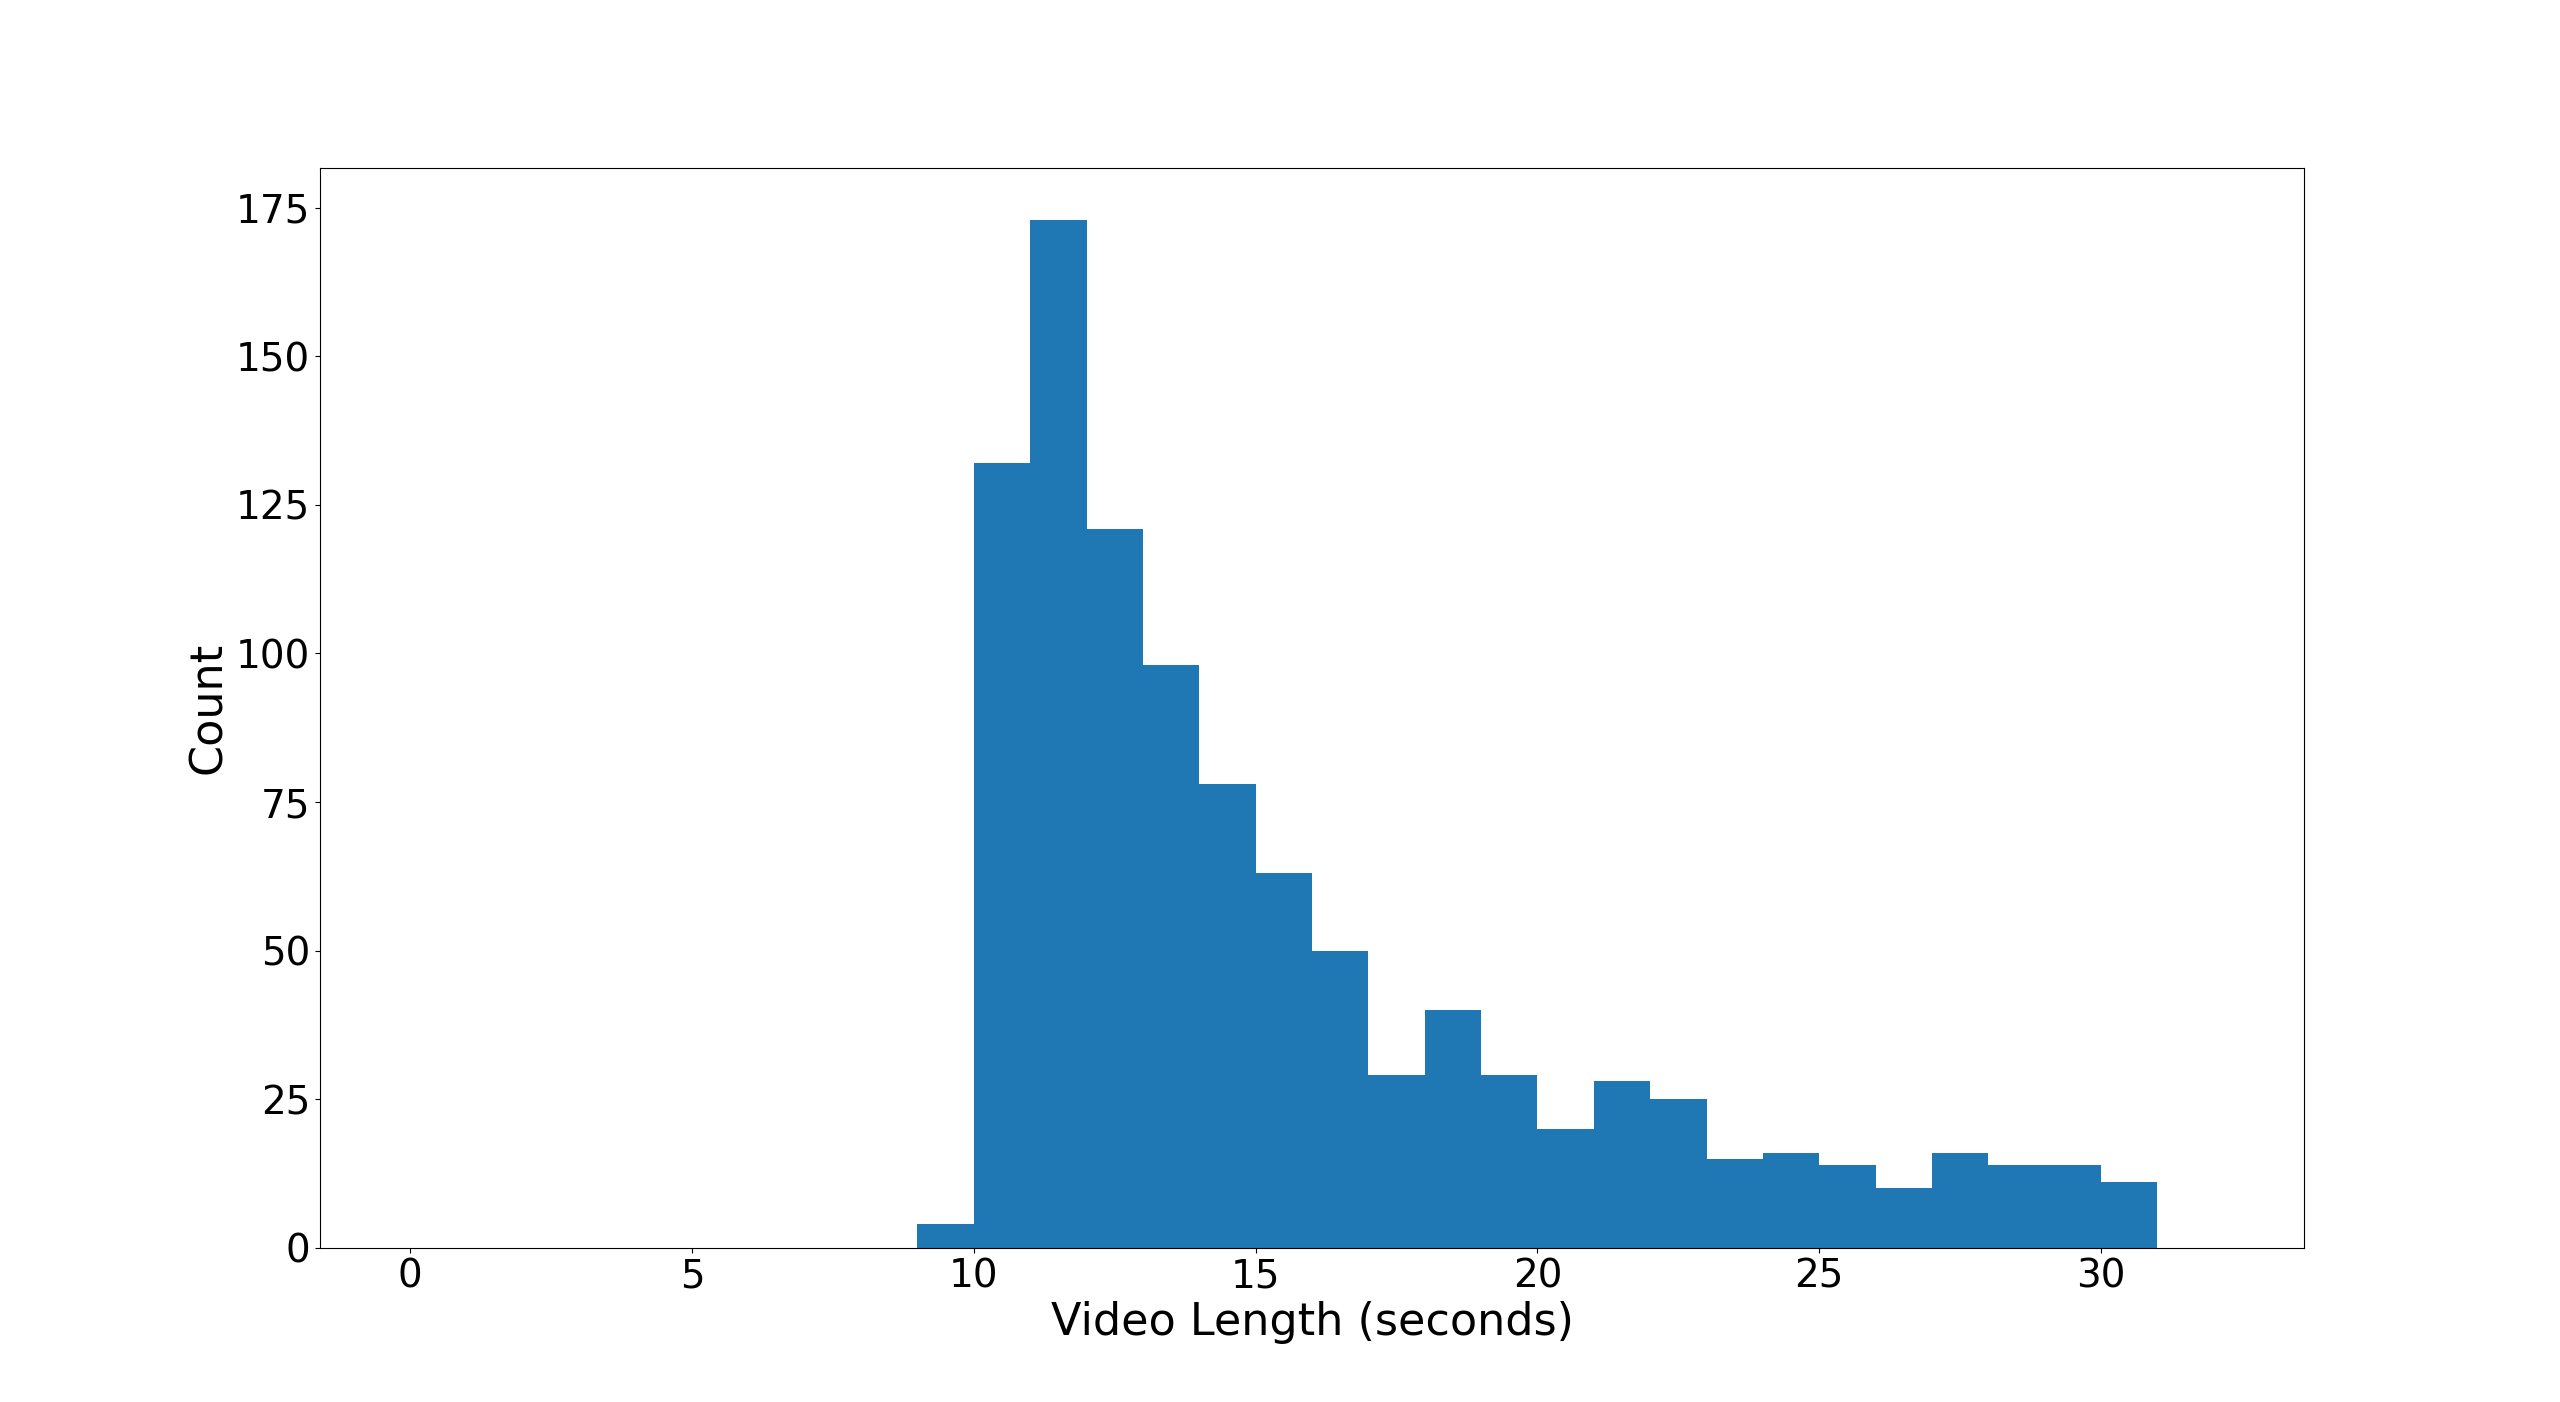
\includegraphics[width=0.7\textwidth]{figures/msr-vtt-length-histogram.png}
      \caption{Length of videos in the MSR-VTT retrieval data split.}
      \label{fig:length_histogram}
\end{figure}

While not used in this paper, other datasets like MSVD \cite{msvd} and ActivityNet \cite{activitynet} are also popular for video understanding tasks.
Microsoft Research Video Description Corpus (MSVD) is similar to MSR-VTT, consisting of short video clips and associated descriptions of the actions in the clip.
MSVD can be used for video captioning, video question answering, and video retrieval.
ActiviyNet is an extremely large dataset used for action classification (human activity understanding).
Given a video, the task is to classify the action being performed in the video, from a set of 200 classes.
ActivityNet version 1.3 contains 19994 videos from YouTube, making it one of the largest video datasets available.
